\documentclass{article}

\usepackage[utf8]{inputenc}
\usepackage[T1]{fontenc}

\usepackage[breaklinks]{hyperref} 
\usepackage{cleveref} 
\usepackage{xcolor} 

\usepackage[electronic]{knowledge}
\knowledgeconfigure{notion, quotation}

\knowledge{url={https://ctan.org/pkg/knowledge}, typewriter}
 | knowledge@package

\knowledge{url={http://mirrors.ctan.org/macros/latex/contrib/knowledge/knowledge.pdf}}
 | documentation

\knowledge{url={https://ctan.org/pkg/hyperref?lang=en}, typewriter}
 | hyperref

\knowledge{text=\LaTeX}
 | latex

\knowledge{notion}
 | Knowledges@concept
 | knowledge@concept
 | knowledges@concept

\knowledge{notion}
 | Directives
 | directives
 | directive

\knowledge{notion, typewriter}
 | notion
 | notions

\knowledge{url={https://en.wikipedia.org/wiki/Tomato}, color=purple, boldface}
 | tomato
 | tomatoes
 | Tomato
 | Tomatoes

\knowledge{notion}
 | introduce
 | introduced
 | introduction

\knowledge{notion}
 | anchor points

\knowledge{notion}
 | composition mode

\knowledge{notion}
 | paper mode

\knowledge{notion}
 | electronic mode

\knowledge{notion}
 | scopes

\knowledgenewrobustcmd\automata{\cmdkl{\mathcal{A}}}

\knowledgenewrobustcmd\interval[2]{
    \cmdkl{[} #1, #2 \cmdkl{]}
}

%%% Custom colors for links

\definecolor{Midnight Green Eagle}{HTML}{005566}
\definecolor{Gamboge}{HTML}{ee9b00}
\definecolor{Ruby Red}{HTML}{9b2226}

\IfKnowledgePaperModeTF{
    %
}{
    % If we are NOT in paper mode (i.e. in composition mode or electronic mode)
    \knowledgestyle{intro notion}{color={Ruby Red}}
    \knowledgestyle{notion}{color={Midnight Green Eagle}}
    \hypersetup{
        colorlinks=true,
        breaklinks=true,
        linkcolor={Midnight Green Eagle}, % Links to sections, pages, etc.
        citecolor={Midnight Green Eagle}, % Links to bibliography
        filecolor={Midnight Green Eagle}, % Links to local file
        urlcolor={Midnight Green Eagle},
    }
}
\IfKnowledgeCompositionModeTF{
    % If we are in composition mode, highlight unknown stuff (in yellow) and display the anchor point.
    \knowledgeconfigure{anchor point color={Ruby Red}, anchor point shape=corner}
    \knowledgestyle{intro unknown}{color={Gamboge}, emphasize}
    \knowledgestyle{intro unknown cont}{color={Gamboge}, emphasize}
    \knowledgestyle{kl unknown}{color={Gamboge}}
    \knowledgestyle{kl unknown cont}{color={Gamboge}}
}{
    %
}

%%% Other packages 

\usepackage{graphicx}
\usepackage{spverbatim}
\usepackage{ulem}


\title{A tutorial for the "knowledge@@package" package}
\author{Enthusiastic users of the "knowledge@@package" package}
\date{\today}


\begin{document}

\maketitle

\begin{abstract}
    This is a tutorial on how to to use the 
    "knowledge@@package" package, together with "knowledge-clustering".
    It shows the basic features of the package, namely how 
    to introduce internal and external hyperlinks on text and math commands,
    as well as more advanced features.
    It also contains a guide on how to install and use "knowledge-clustering", 
    a ``nifty software tool'' that aims to ease the use of "knowledge@@package".
\end{abstract}

\tableofcontents

\paragraph{Acknowledgments} We would like to thank
\href{http://www.matricon.ninja/}{Théo Matricon} for helpful feedback
on a previous version of this document.


\section{Introduction}

\subsection{The "knowledge@@package" package}

The package \AP""knowledge@@package"" is a package for "latex" that helps associating 
information to terms. It can be used for:
\begin{itemize}
    \item managing external urls, for instance separating the file containing   
        the addresses from their use;
    \item managing internal references's such as linking every use of a concept 
        to the place of its introduction
        (in particular avoiding the use of labels);
    \item managing the index in a centralized way;
    \item replacing some macros.
\end{itemize}

Primarily, the goal of "knowledge@@package" is to produce of scientific documents (the longer, the more interesting, such as a thesis or a book) in order to improve their readability on electronic devices. Ultimately, the goal is to produce documents that are more semantic-aware.

\subsection{This tutorial}

This tutorial starts with a description of the \textbf{basic features of
"knowledge@@package"} in \Cref{sec:basic-features}, followed by an
introduction on how to use "knowledge-clustering", which is a
\textbf{command-line tool designed to greatly
speed up the process of writing a document} with "knowledge@@package"
in \Cref{sec:knowledge-clustering}. Finally, \Cref{sec:advanced-features}
deals with more \textbf{advanced features} of the "knowledge@@package" package.

Throughout this document, we will refer to the "knowledge@@package" 
"documentation". It can be accessed locally by
typing \spverb|texdoc knowledge| in 
a prompt or "online@documentation".

\section{Basic features}
\label{sec:basic-features}

Try compiling this document (two compilation phases to have proper links) using \spverb|pdflatex| and see how some notions are hyperlinked to their introduction point (some viewers make it more obvious than others by displaying a preview of the target of a link inside a document).

\subsection{Using "knowledge@@package" in your "latex" document}

To use "knowledge@@package" in your "latex" document, write in the preamble:
\begin{verbatim}
    \usepackage[breaklinks]{hyperref} 
    \usepackage{xcolor} 

    \usepackage{knowledge}

    \knowledgeconfigure{notion, quotation}
\end{verbatim}

By default, "knowledge@@package" is loaded in \AP""composition mode"", which renders 
links and warnings. The document can be switched to \AP""paper mode"",
which is made for printing (links still exist but are displayed in black)
or \AP""electronic mode"" (links are colored, warnings and "anchor points"
are hidden), by writing
\begin{itemize}
    \item \spverb|\usepackage[paper]{knowledge}| or
    \item \spverb|\usepackage[electronic]{knowledge}|.
\end{itemize} 


\subsection{Aesthetical changes and external links}

\AP""Knowledges@@concept"" are the key concept in the "knowledge@@package" 
package. Essentially, a "knowledge@@concept" corresponds to a concept used in 
the document. To invoke a "knowledge@@concept" named ``tomato'', one simply has 
to write \spverb|\kl{tomato}| (or simply
\knowledgeconfigure{quotation=false}%
\spverb|"tomato"|%
\knowledgeconfigure{quotation=true}
if the 'quotation' 
configuration is enabled) in their document. At compilation, this will 
print the text ``tomato'' and apply (aesthetical or semantical) changes that
are associated with the "knowledge@@concept" ``tomato''.

To specify what modifications should be performed on a "knowledge@@concept", 
you must define it, either in the beginning of your document or in an external file (in \texttt{notions.tex} in this example) included in your preamble.
The basic syntax to do so is:
\begin{verbatim}
    \knowledge{}
     | tomato
\end{verbatim}
\AP""Directives"" can be written between the pair of brackets. A complete list of "directives" can be found in \href{https://texlive.mycozy.space/macros/latex/contrib/knowledge/knowledge.pdf#subsection.5.3}{§5.3} of the "knowledge@@package" "documentation". Common "directives" include:
\begin{itemize}
    \item \spverb|url=<LINK>| to add an external hyperlink;
    \item \spverb|color=<COLOR>| to change the color of the "knowledge@@concept";
    \item \spverb|italic| and \spverb|up| to force/unforce italic;
    \item \spverb|boldface| and \spverb|md| to force/unforce boldface;
    \item \spverb|smallcaps| to force small capitals;
    \item \spverb|underline| to underline;
    \item \spverb|lowercase| and \spverb|uppercase| to render the text in lowercase or uppercase;
    \item \spverb|typewriter| to render the text in typewriter;
    \item \spverb|text=<TEXT>| to change the text that is displayed.
\end{itemize}

You will often want to define synonyms, i.e. to have multiple names associated to a single "knowledge@@concept": for instance you might want ``tomatoes'', ``Tomato'' and  ``Tomatoes'' to all refer to the same "knowledge@@concept" as ``tomato''. This can be achieved by defining each synonym on a new line, precedeed by a pipe. For example:
\begin{verbatim}
    \knowledge{url={https://en.wikipedia.org/wiki/Tomato},
        color=olive, boldface}
     | tomato
     | tomatoes
     | Tomato
     | Tomatoes
\end{verbatim}
will produce the following result when one writes \spverb|\kl{Tomatoes}| or
\knowledgeconfigure{quotation=false}%
\spverb|"Tomatoes"|%
\knowledgeconfigure{quotation=true}:%
\begin{quote}
    "Tomatoes"
\end{quote}
namely it will write the text ``Tomatoes'' in bold, olive, and insert a link to the Wikipedia page named ``Tomato''.


\subsection{Internal hyperlinks: the "notion" directive}

The ""notion"" "directive" allows you to easily introduce internal hyperlinks.
Say that you have defined a "knowledge@@concept":
\begin{verbatim}
    \knowledge{notion, <OTHER_DIRECTIVES>}
     | name
     | synonym
\end{verbatim}
By writing \spverb|\intro{name}| (or
\spverb|\intro{synonym}|, or 
\knowledgeconfigure{quotation=false}%
\spverb|""name""|, or \spverb|""synonym""|%
\knowledgeconfigure{quotation=true}%,
) you will \AP""introduce"" your knowledge. Then, whenever you will write
\spverb|\kl{name}| (or
\spverb|\kl{synonym}|, or 
\knowledgeconfigure{quotation=false}%
\spverb|"name"|, or \spverb|"synonym"|)%
\knowledgeconfigure{quotation=true}
"knowledge@@package" will add an internal hyperlink to the place where
your "notion" was "introduced". The default behaviour\footnote{Inherited from
"hyperref".} is to add a link to the beginning of the section in which the "notion" was introduced. Since this is very often unsatisfying, the command
\spverb|\AP| allows you to define custom \AP""anchor points"", depicted as 
small red corners in the left margin of your document when you are in 
"composition mode"\footnote{This document was compiled in "electronic mode" so
the "anchor points" are not shown. However, you can observe "anchor points" in 
the \href{https://github.com/remimorvan/knowledge-examples/tree/main/minimal-example}{minimal example}.}. Internal hyperlinks will refer to the last 
anchor point preceding the "introduction" of your "notion".


By default, "notions" appear in blue, and "introduction" of "notions"
appear in dark blue and italics.
Note that a single "notion" should only be introduced once---even if you have synonyms. Should you want to reintroduce an already introduced "notion", 
you can use the \spverb|\reintro{...}| command.

\subsection{Scopes and extended syntax}

Sometimes the same piece of text can refer to different concepts: for example, in this document, ``knowledge'' refers both to the "knowledge@@package" package
and to the concept of "knowledges@@concept". In this case, \AP""scopes"" allow 
you to distinguish these concepts, by defining the two "knowledges@@concept":
\begin{verbatim}
    \knowledge{url={https://ctan.org/pkg/knowledge}, typewriter}
     | knowledge@package

    \knowledge{notion}
     | knowledge@concept
\end{verbatim}
To invoke one or the other, you can write:
\knowledgeconfigure{quotation=false}%
\begin{verbatim}
    "knowledge@@scope"
        or
    \kl(scope){knowledge}
\end{verbatim}
\knowledgeconfigure{quotation}%
where \spverb|scope| is either \spverb|package| or
\spverb|concept|.
More informations on "scopes" can be found in \href{https://ctan.mines-albi.fr/macros/latex/contrib/knowledge/knowledge.pdf#subsection.3.5}{§3.5} of the "documentation".

Finally, if you want to display some ``text'' that behaves
like some "knowledge@@concept" named ``name'', you can write:
\knowledgeconfigure{quotation=false}%
\begin{verbatim}
    "text@name"
        or
    \kl[name]{text}
\end{verbatim}
\knowledgeconfigure{quotation}%
This is useful when you do not want ``text'' to be a synonym
of ``name'' throughout the paper but only locally.
For instance:
\knowledgeconfigure{quotation=false}%
\begin{verbatim}
    (...) "These vegetables@tomato" are (...)
\end{verbatim}
\knowledgeconfigure{quotation}%
produces:
\begin{quote}
    (...) "These vegetables@tomato" are (...)
\end{quote}
namely the style of the "knowledge@@concept" ``tomato'' is applied to the
string ``These vegetables''.


\subsection{Mathematical commands}
\label{sec:math-commands}


The previous sections can mostly be applied to mathematical commands:
\begin{verbatim}
    $\kl[tomato]{\Pi^P_2}$
\end{verbatim}
will produce $\kl[tomato]{\Pi^P_2}$. However, as a rule of thumb,
this should be avoided as there is a more elegant syntax for 
knowledgyfied mathematical commands. It is recommended to
use semantic macros instead of syntactic ones: for example,
instead of defining a macro \spverb|\Ac| that displays $\mathcal{A}$, 
define \spverb|\automata| or \spverb|\algebra|.

The basic syntax to define a new mathematical command is:
\begin{verbatim}
    \knowledgenewrobustcmd<COMMAND_NAME>{\cmdkl{
        <YOUR_MACRO>
    }}
\end{verbatim}
For example:
\begin{verbatim}
    \knowledgenewrobustcmd\automata{\cmdkl{
        \mathcal{A}
    }}
\end{verbatim}
defines a macro named \spverb|\automata| that prints an `$\mathcal{A}$' and 
defines a "notion" named \spverb|\automata|.
Using the command \spverb|\automata| (e.g: $\automata$) will result in
"knowledge@@package" automatically inserting a link to the last "anchor point"
preceding the introduction of the "notion" \spverb|\automata|.
This notion can be introduced by writing:
\begin{verbatim}
    \intro*\automata
\end{verbatim}
which produces the following result: $\AP\intro*\automata$.

The \spverb|\cmdkl| command allows you to control which part of the macro will be
knowledgyfied/clickable. For instance, if you define the macro:
\AP\phantomintro{\interval}
\begin{verbatim}
    \knowledgenewrobustcmd\interval[2]{
        \cmdkl{[} #1, #2 \cmdkl{]}
    }
\end{verbatim}
then \spverb|$\interval{a}{b}$| will produce $\interval{a}{b}$: only the two
brackets will be clickable.


\section{Knowledge-Clustering}
\label{sec:knowledge-clustering}

\subsection{Goal}

"Knowledge-clustering" is a command-line tool that aims to automate part of
the process of writing a document with "knowledge@@package".
As of today, "knowledge\-clustering" has two main features:
\begin{itemize}
    \item the "clustering" feature, which automates the definitions
    of synonyms. For example,  if at some point you already defined the 
    "knowledge@@concept" \spverb|tomato| and write in your document
    \knowledgeconfigure{quotation=false}%
    \spverb|"Tomatoes"|
    \knowledgeconfigure{quotation}%
    then, at compilation, "latex" will rightfully produce a warning,
    saying that the knowledge \spverb|Tomatoes| is undefined.
    At this point, you should run "knowledge-clustering", which will suggest to 
    you to define \spverb|Tomatoes| as a synonym of \spverb|tomato|.
    \item the "add quotes" feature, that can be used at the very end of your 
    writing process, to check if every piece of text that is defined as
    a "knowledge@@concept" is surronded by quotes. For example, this feature 
    \knowledgeconfigure{quotation=false}%
    would suggest to replace the string \spverb|Let $x$ be a tomato such that (…)|
    in you \spverb|.tex| file by \spverb|Let $x$ be a "tomato" such that (…)|.
    \knowledgeconfigure{quotation}%
\end{itemize}

\subsection{Installation}

To install "knowledge-clustering", you need to have a machine with
\spverb|python3| and \spverb|pip3|. To install, or upgrade, "knowledge-clustering",
you can simply run
\begin{verbatim}
    pip3 install --upgrade knowledge-clustering
\end{verbatim}
in your shell.
Then, you should run
\begin{verbatim}
    knowledge init
\end{verbatim}
to download some data (roughly 35Mb), used by the "clustering" algorithm\footnote{This 
downloads some data used by "NLTK", a natural language package used by 
"knowledge@@package".}.

\paragraph{Autocomplete}
If the autocomplete of the command \spverb|knowledge| does not work,
you can follow the following procedure:
if you are using \spverb|zsh| (resp. \spverb|bash|), then add
\knowledgeconfigure{quotation=false}%
\begin{verbatim}
    eval "`pip completion --zsh`"
\end{verbatim}
or 
\begin{verbatim}
    eval "`pip completion --bash`"
\end{verbatim}
\knowledgeconfigure{quotation}%
in your \spverb|.zshrc| file (resp. \spverb|.bashrc|).
For the change to take effect, you either need to launch a new terminal
or run \spverb|source ~/.zshrc| (resp. \spverb|source ~/.bashrc|).

\subsection{Clustering knowledges}

\subsubsection{Basic use}

The \AP""clustering"" feature is meant to be used
when you are writing your "latex" document with "knowledge@@package".
Maintaining the list of all the "knowledges@@concept" you are using
can be burdersome, so usually you will write your "latex" code
and use, in this code, some "knowledges@@concept" that are yet to be
defined.

\begin{figure}[htb]
    \centering
    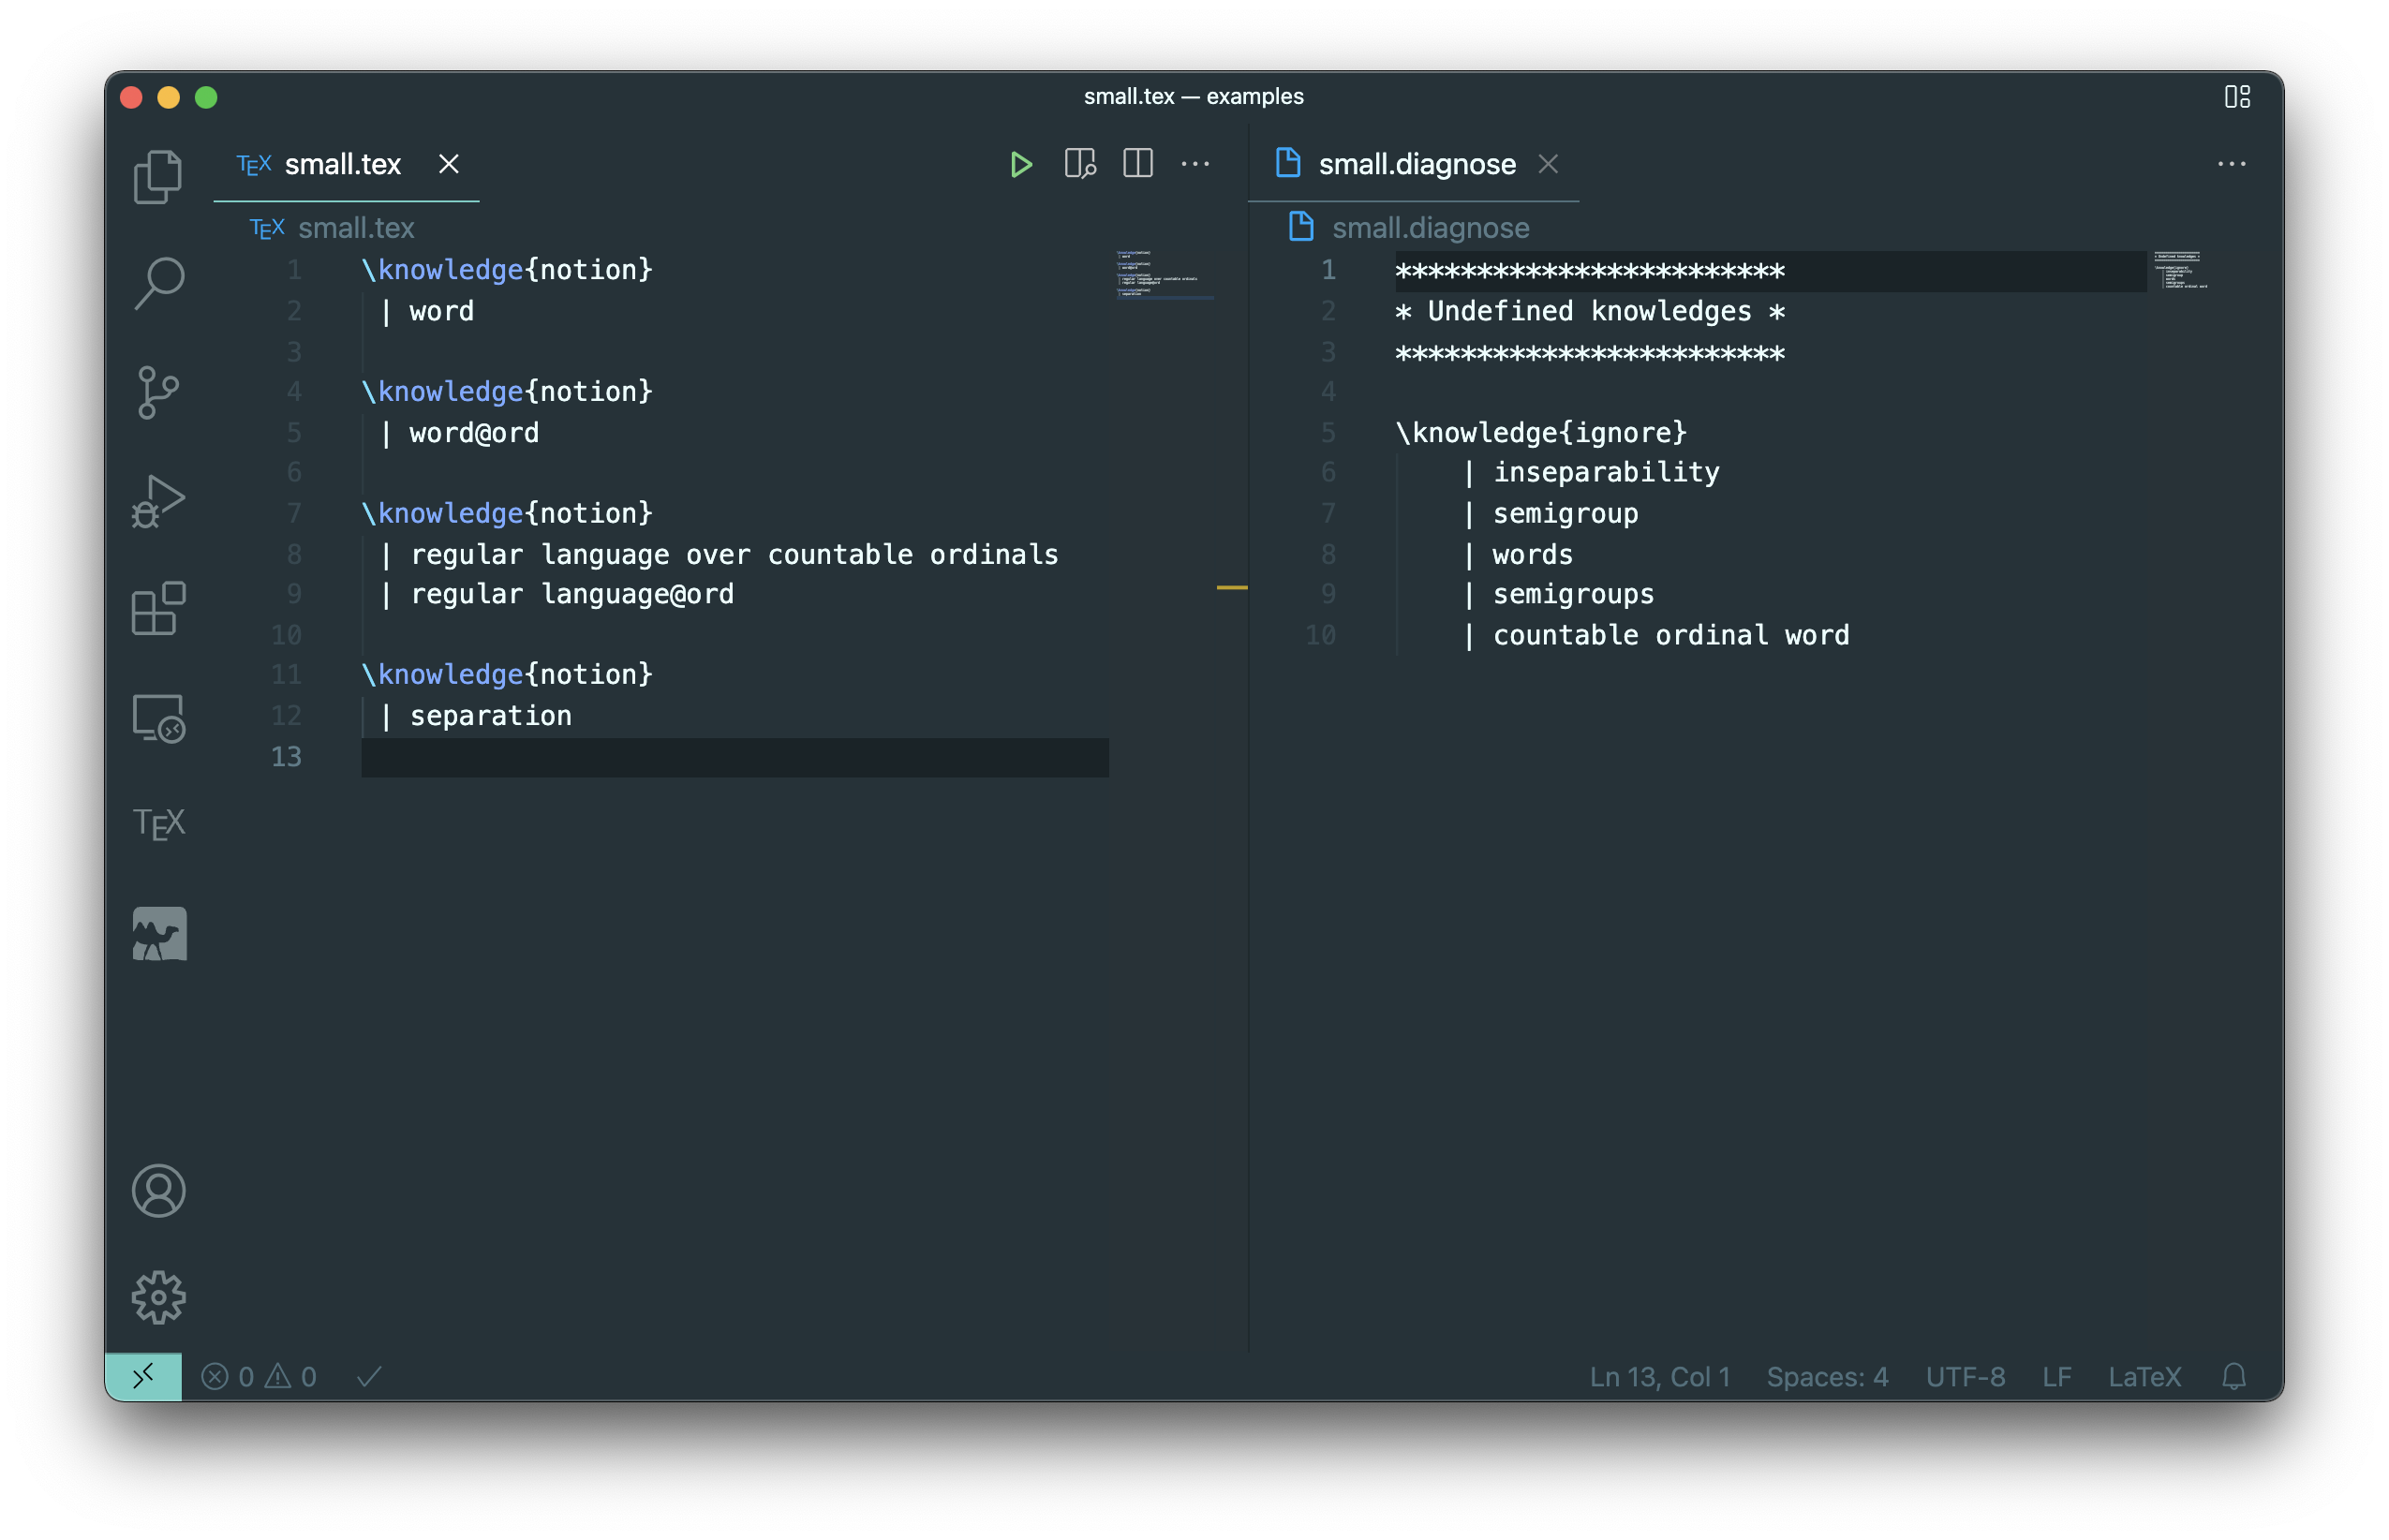
\includegraphics[width=.95\textwidth]{img/small-before.png}
    \caption{%
        \label{fig:clustering-before}
        Content of the file containing the defined "knowledges@@concept"
        (left-hand side) and of the \texttt{.diagnose} file produced by
        "latex" at compilation (right-hand side), before running 
        "knowledge-clustering".
    }
\end{figure}

For example, \Cref{fig:clustering-before} illustrates the following situation:
in the file containing all your defined "knowledges@@concept", you have
four "knowledges@@concept", one of which is ``\spverb|word|''.
In your main \spverb|.tex| file---which is not reproduced here---, you used some 
undefined "knowledges@@concept", such as ``\spverb|words|'' and
``\spverb|semigroup|''.
At compilation, "latex" will produce a warning, saying that you have undefined
"knowledges@@concept" and write in a \spverb|.diagnose| file a list
of these undefined "knowledges@@concept".

At this point, you have two options: you can either define every undefined "knowledge@@concept", by hand, and say that ``\spverb|words|'' is a synonym of
``\spverb|word|'' while ``\spverb|semigroup|'' is a new "knowledge@@concept".
Or, you can use the "clustering" feature of "knowledge-clustering": feed
it both files (the file \spverb|small.tex| containing the defined 
"knowledges@@concept" and
the \spverb|small.diagnose| file containing the undefined "knowledges@@concept")
by running the command
\begin{verbatim}
    knowledge cluster -k small.tex -d small.diagnose
\end{verbatim}
which will write suggestions in your file \spverb|small.tex|,
as depicted in \Cref{fig:clustering-after}. These suggestions
take the form of comments: if you agree with the suggestion, you can just
uncomment the line and otherwise, you should move it, by hand.

\begin{figure}[htb]
    \centering
    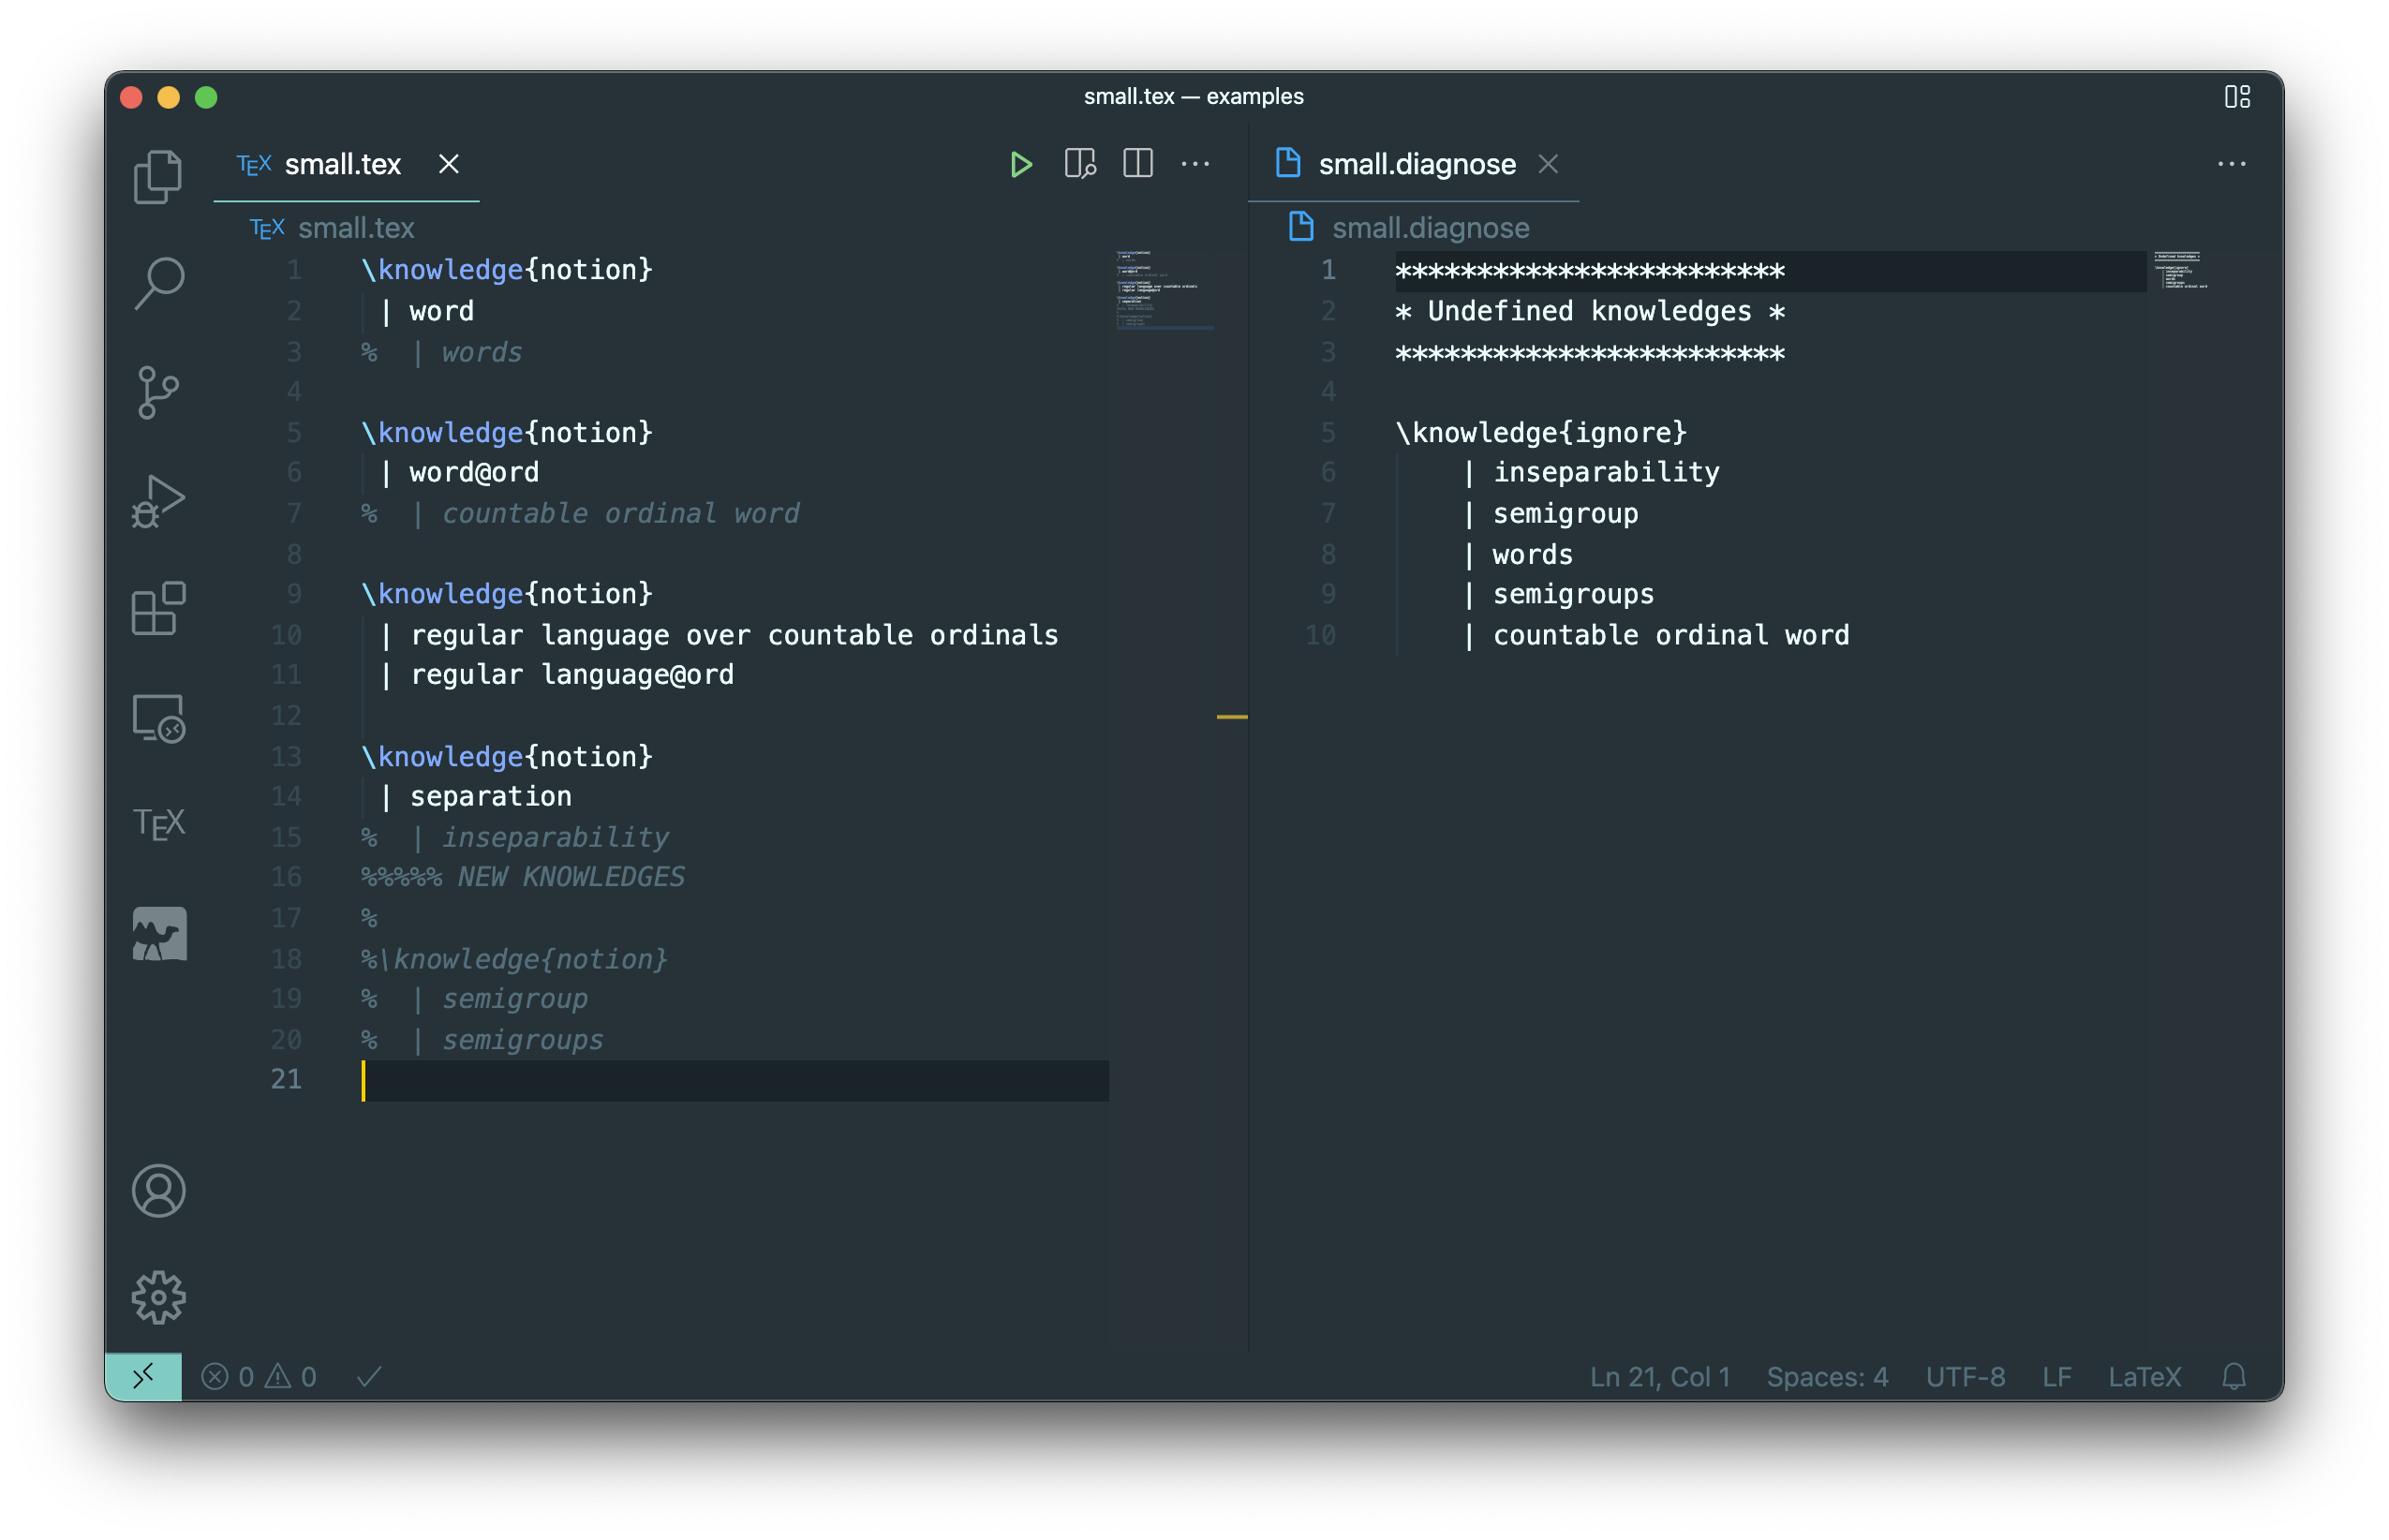
\includegraphics[width=.95\textwidth]{img/small-after.png}
    \caption{%
        \label{fig:clustering-after}
        After running "knowledge-clustering", the \texttt{small.diagnose} file
        is left unchanged, while \texttt{small.tex} now contains suggestions
        of how to define the new "knowledges@@concept".
     }
\end{figure}


\subsubsection{Advanced features}

To display the help, you can run \spverb|knowledge cluster --help|.

\paragraph{Language} The "clustering" algorithm relies on natural language 
processing and is language-specific. As of today, only two languages
are supported: english (which is the default language) and french.
To use "knowledge-clustering" on a document written in french,
simply add \spverb|-l fr| or \spverb|--lang fr| at the end of your command.


\paragraph{Scopes} In the example of
\Cref{fig:clustering-before,fig:clustering-after}
you can see that "knowledge-cluste\-ring" inferred that the
scope ``ord'' meant ``countable ordinals''\footnote{This was inferred
by reading the \texttt{small.tex} file and was used to cluster
the "knowledge@@concept" ``countable ordinal word'' with ``word@ord''.}.
If you want the list of scopes it saw
and their inferred meaning, you can use the \spverb|-S| or \spverb|--scope| 
option. 
For instance, running:
\begin{verbatim}
    knowledge cluster -k small.tex -d small.diagnose --scope
\end{verbatim}
will print in your prompt
\begin{verbatim}
    Defined scopes:
	    @ord : [['ordinals', 'countable'], ['ord']]
\end{verbatim}


\subsection{Forgotten quotes}


The "add quotes" feature is meant to be used when your document is (nearly)
finished and you want to check that you have not forgotten quotes symbols
(or a \spverb|kl{}| command) before and after defined "knowledges@@concept".

The basic syntax is the following:
\begin{verbatim}
    knowledge addquotes -t <TEX_FILE> -k <NOTION_FILE> 
\end{verbatim}
where:
\begin{itemize}
    \item \texttt{<TEX\_FILE>} is the \spverb|.tex| file containing your "latex"
    document;
    \item \texttt{<NOTION\_FILE>} is the file containing the
    "knowledges@@concept" you have defined.
\end{itemize}
Then, your prompt will display something like
\begin{verbatim}
    Found a match for `blabla` at line 41.
    Add quotes? [y/n]
\end{verbatim}
Depending on your answer, the "add quotes" feature will add a quote
\knowledgeconfigure{quotation=false}%
\spverb|"| before, and a quote \spverb|"| after 
\knowledgeconfigure{quotation}%
the piece of text ``blabla'' found at line 41.

If you want more precision,
you can also print the columns (a tabulation counting as 4 columns)
using the option \spverb|-c| or \spverb|--column|.
\begin{spverbatim}
    Found a match for `blabla` between line 41, column 13 and line 41, column 19.
    Add quotes? [y/n]
\end{spverbatim}

Finally, the option \spverb|-F| or \spverb|--force| adds
quote symbols around every match, without asking your consent first.
It is \textbf{highly discouraged} to use this option. 

\subsection{Contributing to "knowledge-clustering"}

If you have bugs to report or suggestions, you can submit a
\href{https://github.com/remimorvan/knowledge-clustering/issues}{new issue},
or a \href{https://github.com/remimorvan/knowledge-examples/pulls}{new pull} 
request on \href{https://github.com/remimorvan/knowledge-examples}{github}, or get in touch by email with
one of the maintainers.


\section{Advanced features}
\label{sec:advanced-features}

This section is dedicated on more advanced features of "knowledge@@package".

\subsection{Changing the default colors}

By default, "knowledge@@package" will print notions in blue and
introductions of notions in dark blue if the document is compiled
in "composition mode" or "electronic mode", but the external hyperlinks
will still be printed in black. Moreover, if it is in
"composition mode", undefined "knowledges@@concept" will appear in yellow,
and anchor points in red.

Unfortunately, the default colors are \sout{ugly} not maximizing the aesthetical potential of your "latex" document.
Using \verb|\knowledgestyle| (\href{https://distrib-coffee.ipsl.jussieu.fr/pub/mirrors/ctan/macros/latex/contrib/knowledge/knowledge.pdf#subsubsection.3.3.4}{§3.3.4} of the "documentation"), you can customise these colors. Moreover,
\verb|\hypersetup| from the "hyperref" package lets you change the colors of
external hyperlinks. Finaly, using
\begin{verbatim}
    \knowledgeconfigure{anchor point color={…}}
\end{verbatim}
lets detailed-oriented users change the color of "anchors points".
However, you want some of these changes to only take effect when you are in
"paper mode", "electronic mode" or "composition mode"\footnote{Fun fact:
the "paper mode" is used by \href{https://www.dagstuhl.de/en/publications/lipics}{LIPIcs} when compiling proceedings. Should you decide
to color your links even in "paper mode", you might make Dagstuhl annoyed.}:
this can be achieved using the commands:
\begin{verbatim}
    \IfKnowledgePaperModeTF{…}{…}
    \IfKnowledgeCompositionModeTF{…}{…}
\end{verbatim}

For example, this document was produced using the following configuration:
\begin{spverbatim}
    \definecolor{Midnight Green Eagle}{HTML}{005566}
    \definecolor{Gamboge}{HTML}{ee9b00}
    \definecolor{Ruby Red}{HTML}{9b2226}

    \IfKnowledgePaperModeTF{
        %
    }{
        % If we are NOT in paper mode (i.e. in composition mode or electronic mode)
        \knowledgestyle{intro notion}{color={Ruby Red}}
        \knowledgestyle{notion}{color={Midnight Green Eagle}}
        \hypersetup{
            colorlinks=true,
            breaklinks=true,
            linkcolor={Midnight Green Eagle}, % Links to sections, pages, etc.
            citecolor={Midnight Green Eagle}, % Links to bibliography
            filecolor={Midnight Green Eagle}, % Links to local file
            urlcolor={Midnight Green Eagle},
        }
    }
    \IfKnowledgeCompositionModeTF{
        % If we are in composition mode, highlight unknown stuff (in yellow) and display the anchor point.
        \knowledgeconfigure{anchor point color={Ruby Red}, anchor point shape=corner}
        \knowledgestyle{intro unknown}{color={Gamboge}, emphasize}
        \knowledgestyle{intro unknown cont}{color={Gamboge}, emphasize}
        \knowledgestyle{kl unknown}{color={Gamboge}}
        \knowledgestyle{kl unknown cont}{color={Gamboge}}
    }{
        %
    }
\end{spverbatim}

This produces the following rust: in "composition mode",
every link (both internal and external) appears in 
a nice shade of blue, called ``Midnight Green Eagle'', definitions and "anchor 
points" are displayed in dark red (``Ruby Red''), and unknown 
"knowledges@@concept" are displayed in dark yellow (``Gamboge'').
In "electronic mode", everything works the same except that
"anchor points" are not displayed and unknown "knowledges@@concept" are 
not highlighted. Finally, in "paper mode", everything is printed in black.

\subsection{Weird spacing in math commands}

Say you want to define a binary relation: without "knowledge@@package"
you would write something like:
\begin{verbatim}
    \newrobustcmd{\myrelation}{%
        \mathrel{\mathcal{R}}%
    }
\end{verbatim}
which will have the desired behaviour: writting
\verb|$x \myrelation y$| will produce $x \myrelation y$
(i.e. the relation symbol is precedeed and followed by spaces),
and writting \verb|let $\myrelation$ be a relation|
produces ``let $\myrelation$ be a relation'': everything works as
expected. Now try to knowledgify this command, by defining it like:
\begin{verbatim}
    \knowledgenewrobustcmd{\myklrelation}{%
        \mathrel{\cmdkl{\mathcal{R}}}%
    }
\end{verbatim}
which will produce $x \myklrelation y$ and ``let $\myklrelation$ be a 
relation''\footnote{You can observe here a fun phenomenon: if a 
"knowledge@@concept" is defined but not introduced, it will still be displayed 
in blue---but it will not be clickable.}. The command does not behave as 
expected in the second case! This is because of the definition of
\spverb|\knowledgenewrobustcmd| (see \href{https://distrib-coffee.ipsl.jussieu.fr/pub/mirrors/ctan/macros/latex/contrib/knowledge/knowledge.pdf#subsubsection.3.9.1}{§3.9.1} of the "documentation"), which is essentially equivalent to:
\begin{verbatim}
    \newrobustcmd\myklrelation{%
        \withkl{\kl[\myklrelation]}{%
            \mathrel{\cmdkl{\mathcal{R}}}
        }
    }
    \knowledge{\myklrelation}{notion}
\end{verbatim}
To obtain the desired behaviour, one has to change the position
of the \verb|\mathrel| command like so:
\begin{verbatim}
    \newrobustcmd\mynewklrelation{%
        \mathrel{%
            \withkl{\kl[\mynewklrelation]}{%
                \cmdkl{\mathcal{R}}
            }%
        }%
    }
    \knowledge{\mynewklrelation}{notion}
\end{verbatim}
which produces the following result:
$x \mynewklrelation y$ and ``let $\mynewklrelation$ be a relation''.
More details can be found in \href{https://distrib-coffee.ipsl.jussieu.fr/pub/mirrors/ctan/macros/latex/contrib/knowledge/knowledge.pdf#subsubsection.3.9.2}{§3.9.2} of the "documentation".

\subsection{Other functionalities}

This tutorial is far from being exhaustive: you can take a look at
the "documentation" to see all the possible wonders "knowledge@@package" has
to offer, such as \href{https://mirror.ibcp.fr/pub/CTAN/macros/latex/contrib/knowledge/knowledge.pdf#subsubsection.3.8.3}{handling indexes}, \href{https://mirror.ibcp.fr/pub/CTAN/macros/latex/contrib/knowledge/knowledge.pdf#subsubsection.3.9.3}{knowledgifying already-defined commands}, \href{https://mirror.ibcp.fr/pub/CTAN/macros/latex/contrib/knowledge/knowledge.pdf#subsubsection.3.9.3}{defining command behaving diffently depending on whether they are used in text or math mode}, etc. 

\end{document}